\providecommand{\relativeRoot}{../..}
\documentclass[\relativeRoot/main.tex]{subfiles}
\graphicspath{{figures/}}

\begin{document}

\section{Results}
\label{sec:dataset:results}

In this section, we summarize selected findings. To that end, LNL involvement based on \gls{ct}, \gls{mri}, \gls{pet} and \gls{fna} was converted into a consensus decision via a logical OR, i.e. a \gls{lnl} is considered involved if it was positive for one of these 4 modalities. However, only a small fraction of the information contained in the full dataset can be summarized here in tables. Thus, the interested reader is encouraged to explore the full dataset directly.

\subsection*{Graphical user interface}

\Cref{fig:dataset:gui_screenshot} shows the \gls{gui} for analyzing the dataset. The main patient characteristics (smoking status, \gls{hpv} status, and primary treatment) are shown on the top left. In the bottom-left panel, the user can specify characteristics of the primary tumor. In the example, the user considers all subsites combined, but restricts the patient selection to late T-category tumors (T3/T4) that extend over the midsagittal plane. On the top-right, the user selected the diagnostic modalities \gls{ct}, \gls{mri}, \gls{pet} and \gls{fna}, which are connected via a logical OR, i.e. a lymph node level is considered as involved for a patient if it was considered positive for at least one of the modalities available for that patient. The main panel shows the involvement of \glspl{lnl}. In the example, the user restricts the selection to patients with positive ipsilateral level III while all other levels are unspecified. In total, 38 out of 287 patients meet these selection criteria. The main panel now displays the number of patients with involvement of the other levels. E.g. 21 patients have contralateral level II involved, and 12 patients ipsilateral level IV.

\begin{figure}
    \centering
    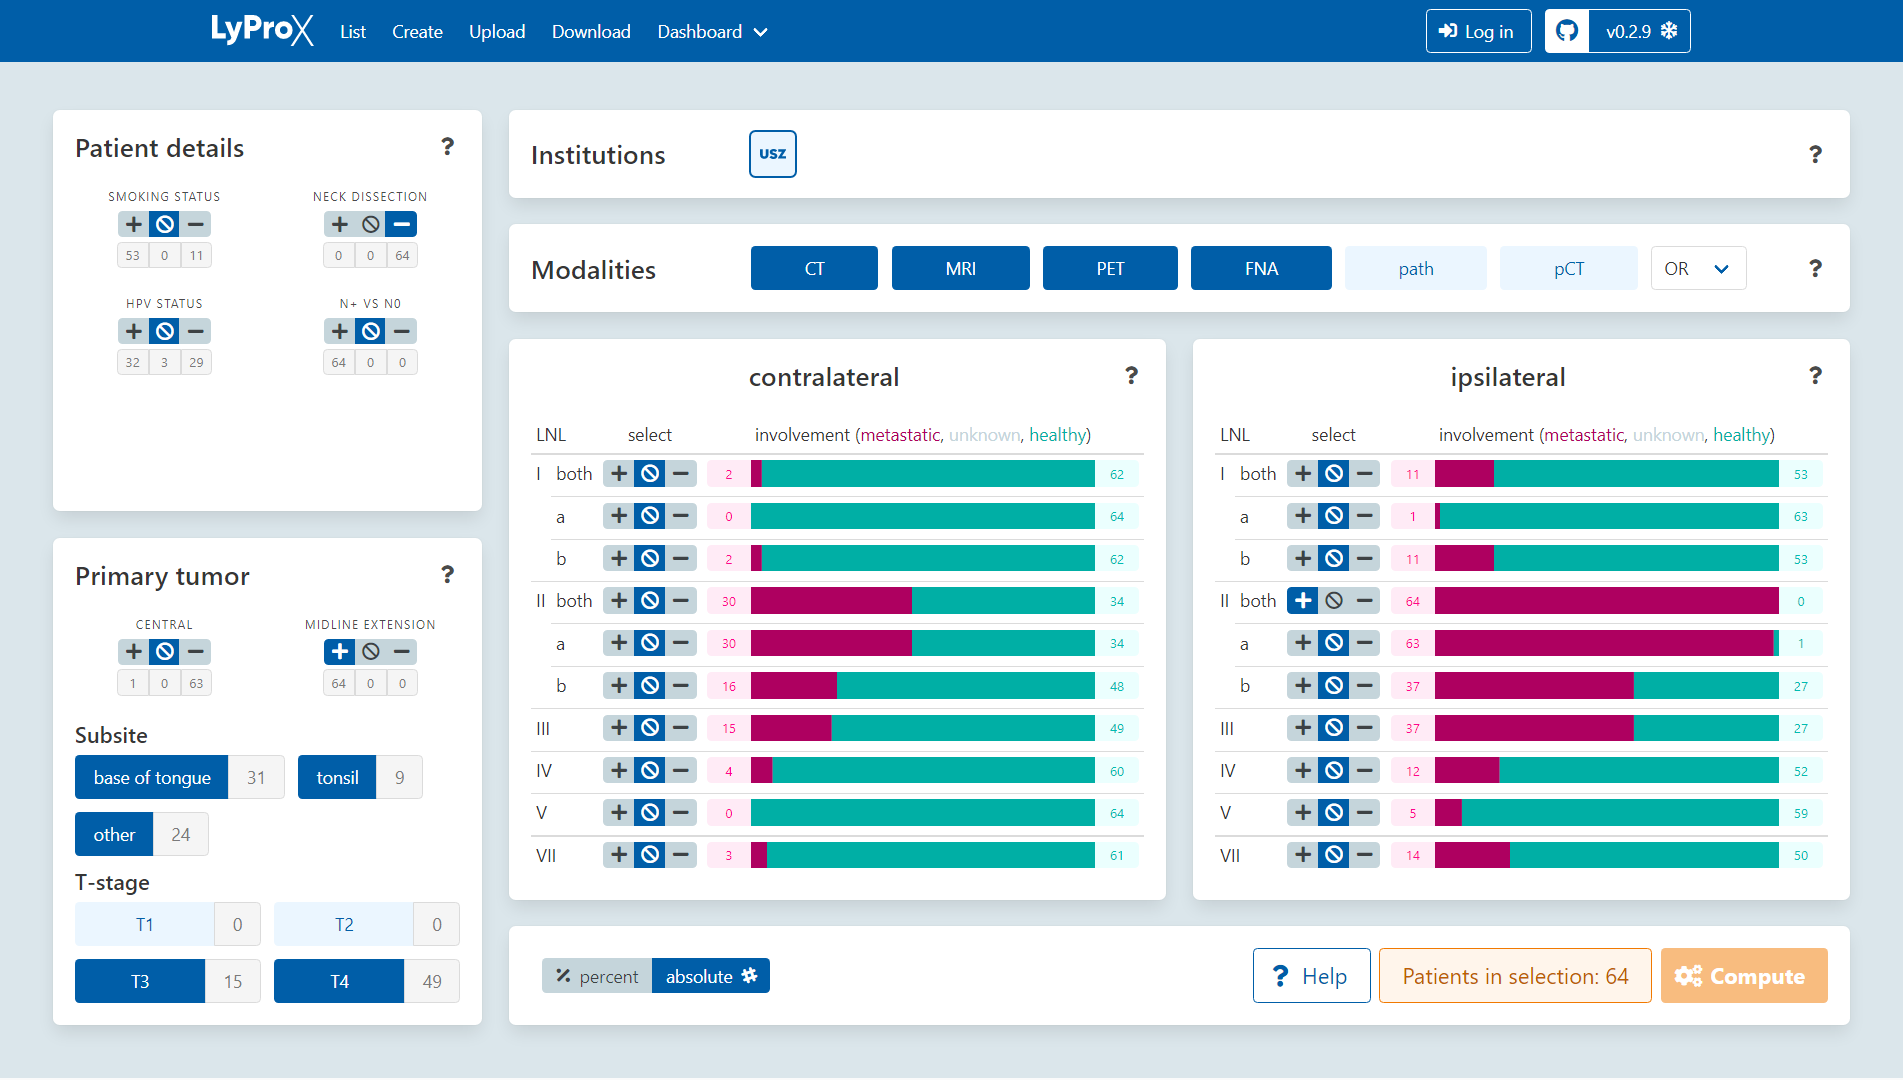
\includegraphics[width=1.0\textwidth]{gui_screenshot.png}
    \caption{Graphical user interface to analyze lymphatic metastatic progression patterns.}
    \label{fig:dataset:gui_screenshot}
\end{figure}

\subsection*{Prevalence}

Overall prevalence of lymph node level involvement is reported in \cref{table:dataset:prevalence} and visualized in \cref{fig:dataset:statistics} panel a and b.

\begin{table}[!ht]
    \centering
    \caption{
        Prevalence of LNL involvement for the whole patient cohort (all) and stratified according to early (T1/T2) versus late (T3/T4) T-category and HPV positive (HPV + ) versus HPV negative (HPV-) tumors. For each LNL, the first column indicates the number of patients showing involvement in the level, the second column the percentage of positive patients in the respective group.
    }
    \resizebox*{\textwidth}{!}{
        \begin{tabular}{|ll||c|rr|rr|rr|rr|rr|rr|}
        \hline
            \multicolumn{2}{|c||}{} & n & \multicolumn{2}{|c|}{I} & \multicolumn{2}{|c|}{II} & \multicolumn{2}{|c|}{III} & \multicolumn{2}{|c|}{IV} & \multicolumn{2}{|c|}{V} & \multicolumn{2}{|c|}{VII} \\
            \hline \hline
            \multirow{9}{*}{\rotatebox[origin=c]{90}{ipsi}} & all & 287 & 30 & 10\% & 232 & 81\% & 113 & 39\% & 31 & 11\% & 16 & 6\% & 30 & 10\% \\
            & T1/T2 & 150 & 10 & 7\% & 118 & 79\% & 48 & 32\% & 10 & 7\% & 4 & 3\% & 12 & 8\% \\
            & T3/T4 & 137 & 20 & 15\% & 114 & 83\% & 65 & 47\% & 21 & 15\% & 12 & 9\% & 18 & 13\% \\
            & HPV$+$ & 181 & 20 & 11\% & 155 & 86\% & 73 & 40\% & 20 & 11\% & 12 & 7\% & 18 & 10\% \\
            & HPV$-$ & 96 & 8 & 8\% & 69 & 72\% & 37 & 39\% & 11 & 11\% & 4 & 4\% & 12 & 13\% \\
            & HPV$+$, T1/T2 & 100 & 7 & 7\% & 86 & 86\% & 35 & 35\% & 8 & 8\% & 3 & 3\% & 10 & 10\% \\
            & HPV$+$, T3/T4 & 81 & 13 & 16\% & 69 & 85\% & 38 & 47\% & 12 & 15\% & 9 & 11\% & 8 & 10\% \\
            & HPV$-$, T1/T2 & 43 & 2 & 5\% & 27 & 63\% & 11 & 26\% & 2 & 5\% & 1 & 2\% & 2 & 5\% \\
            & HPV$-$, T3/T4 & 53 & 6 & 11\% & 42 & 79\% & 26 & 49\% & 9 & 17\% & 3 & 6\% & 10 & 19\% \\
            \hline
            \multirow{5}{*}{\rotatebox[origin=c]{90}{contra}} & all & 287 & 3 & 1\% & 51 & 18\% & 21 & 7\% & 7 & 2\% & 2 & 1\% & 6 & 2\% \\
            & T1/T2 & 150 & 0 & 0\% & 13 & 9\% & 4 & 3\% & 2 & 1\% & 1 & 1\% & 1 & 1\% \\
            & T3/T4 & 137 & 3 & 2\% & 38 & 28\% & 17 & 12\% & 5 & 4\% & 1 & 1\% & 5 & 4\% \\
            & HPV$+$ & 181 & 3 & 2\% & 26 & 14\% & 13 & 7\% & 6 & 3\% & 2 & 1\% & 3 & 2\% \\
            & HPV$-$ & 96 & 0 & 0\% & 25 & 26\% & 8 & 8\% & 1 & 1\% & 0 & 0\% & 3 & 3\% \\
        \hline
        \end{tabular}
    }
    \label{table:dataset:prevalence}
\end{table}

\subsection*{Dependence on T-category}

\Cref{table:dataset:prevalence} and \cref{fig:dataset:statistics} panels a and b compare the prevalence of \gls{lnl} involvement for early (T1/T2) versus late (T3/T4) T-category-patients. Consistent with common intuition, higher involvement was observed for late T-categories. Involvement of ipsilateral level II was high also for T1/T2 \& (79\%) and therefore increased only moderately for T3/T4 \& (83\%). However, involvement of the downstream levels III, IV, V increased from 32\%, 7\%, 3\% for early T-category patients to 47\%, 15\%, 9\% for late T-category. On the contralateral side, involvement of levels II, III, IV, V increased from 9\%, 3\%, 1\%, 1\% for T1/T2 patients to 28\%, 12\%, 4\%, 1\% for T3/T4.

\begin{figure}
    \centering
    \def\svgwidth{1.0\textwidth}
    \input{figures/statistics.pdf_tex}
    \caption{(a) Contralateral and (b) ipsilateral prevalence of \gls{lnl} involvement for the whole patient cohort and stratified according to early (T1/T2) versus late (T3/T4) T-category. Contralateral \gls{lnl} involvement stratified according to (c) midsagittal plan extension and (d) involvement of ipsilateral level III. Ipsilateral \gls{lnl} involvement stratified according to HPV status for T1/T2 tumors (e) and T3/T4 tumors (f).}
    \label{fig:dataset:statistics}
\end{figure}

\subsection*{Dependence on upstream levels}

\begin{table}[!ht]
    \centering
    \caption{
        Simultaneous involvement in levels II, III, and IV and frequency of skip metastases, for the whole patient cohort (all) and stratified according to early (T1/T2) versus late (T3/T4) T-category. Columns 1-3 define the 8 possible combinations of involvement; subsequent columns report the number of patients with the respective combination of co-involved levels.
    }
    \resizebox*{\textwidth}{!}{
        \begin{tabular}{|ccc|rr|rr|rr|rr|rr|rr|}
            \hline
            \multicolumn{3}{|c|}{~} & \multicolumn{6}{c}{ipsi} & \multicolumn{6}{|c|}{contra} \\
            II & III & IV & \multicolumn{2}{c}{all} & \multicolumn{2}{c}{T1/T2} & \multicolumn{2}{c}{T3/T4} & \multicolumn{2}{|c}{all} & \multicolumn{2}{c}{T1/T2} & \multicolumn{2}{c|}{T3/T4} \\ 
            \hline \hline
            $+$ & $+$ & $+$ &  28 & 10\% &  8 &  5\% & 20 & 15\% &   5 &  2\% &   1 &  1\% &  4 &  3\% \\
            $+$ & $+$ & $-$ &  80 & 28\% & 37 & 25\% & 43 & 31\% &  13 &  5\% &   2 &  1\% & 11 &  8\% \\
            $+$ & $-$ & $+$ &   2 &  1\% &  2 &  1\% &  0 &  0\% &   0 &  0\% &   0 &  0\% &  0 &  0\% \\
            $+$ & $-$ & $-$ & 122 & 43\% & 71 & 47\% & 51 & 37\% &  33 & 11\% &  10 &  7\% & 23 & 17\% \\
            $-$ & $+$ & $+$ &   0 &  0\% &  0 &  0\% &  0 &  0\% &   1 &  0\% &   1 &  1\% &  0 &  0\% \\
            $-$ & $+$ & $-$ &   5 &  2\% &  3 &  2\% &  2 &  1\% &   2 &  1\% &   0 &  0\% &  2 &  1\% \\
            $-$ & $-$ & $+$ &   1 &  0\% &  0 &  0\% &  1 &  1\% &   1 &  0\% &   0 &  0\% &  1 &  1\% \\
            $-$ & $-$ & $-$ &  49 & 17\% & 29 & 19\% & 20 & 15\% & 232 & 81\% & 136 & 91\% & 96 & 70\% \\
            \hline
            \multicolumn{3}{|c|}{~} & 287 & ~ & 150 & ~ & 137 & ~ & 287 & ~ & 150 & ~ & 137 & ~	\\
            \hline
        \end{tabular}
    }
    \label{table:dataset:upstream}
\end{table}

\Cref{table:dataset:upstream} considers the frequency of involvement in downstream levels depending on the involvement in upstream levels. On the ipsilateral side, level III harbored metastases in 47\% of patients (108 out of 232) when level II was positive, but in only 9\% of patients (5 out of 55) when II was negative. Analogously, level IV harbored metastases in 25\% of patients (28 out of 118) when level III was positive, but in only 2\% of patients (3 out of 174) when III was negative (Fig. 3). On the contralateral side, level III harbored metastases in 35\% of patients (18 out of 51) when level II was positive, but in only 1\% of patients (3 out of 236) when II was negative.

\subsection*{Contralateral involvement}

Apart from late T-category (\cref{table:dataset:upstream}), extension of the primary tumor across the midsagittal plane and higher ipsilateral involvement was associated with higher contralateral involvement. \cref{table:dataset:contralateral} reports the prevalence of contralateral lymph node involvement depending on three factors: T-category, midsagittal extension, and whether ipsilateral level III was involved. For all 197 patients without midline extension, contralateral involvement in levels II, III, IV, V was 10\%, 3\%, 2\%, 1\% compared to 36\%, 18\%, 4\%, 0\% with midline extension (90 patients). In addition, out of 38 patients with late T-category, midsagittal extension, and positive ipsilateral level III, 21 \& (55\%) showed contralateral involvement in level II and 12 \& (32\%) in level III. Out of 39 late T-category patients with midsagittal extension but negative ipsilateral level III, contralateral involvement was lower (24\% in level II, 7\% in level III). In \cref{table:dataset:contralateral}, we consider ipsilateral level III rather than II, because level II is involved in 81\% of all patients. However, when ipsilateral level II is not involved, contralateral involvement is unlikely (1 out of 55 patients showed metastases in contralateral level II). We further note that the three factors considered in \cref{table:dataset:contralateral} are correlated. Out of 150 early T-category patients, 11 \& (7\%) showed midline extension, whereas 79 \& (58\%) out of 137 late T-category patients showed midline extension. As expected, contralateral involvement depended on primary tumor subsite. When considering only primary tumors strictly restricted to the tonsils (118 patients), contralateral involvement in levels II and III was 8\% and 3\%, respectively.

\begin{table}[!hb]
    \centering
    \caption{
        Risk factors for contralateral involvement. Columns 1-3 define the 8 possible combinations of positive/negative mid-sagittal plan extension, late/early T-category, and positive/negative involvement of ipsilateral level III. Subsequent columns report the number of patients and percentages with involvement in the respective level for each combination of risk factors.
    }
    \resizebox*{\textwidth}{!}{
        \begin{tabular}{|ccc||r|rr|rr|rr|rr|rr|rr|}
            \hline
            T-stage & midline & ipsi III & n & \multicolumn{2}{|c|}{I} & \multicolumn{2}{|c|}{II} & \multicolumn{2}{|c|}{III} & \multicolumn{2}{|c|}{IV} & \multicolumn{2}{|c|}{V} & \multicolumn{2}{|c|}{VII} \\ 
            \hline \hline
            early & no & $-$ & 94 & 0 & 0\% & 4 & 4\% & 2 & 2\% & 1 & 1\% & 0 & 0\% & 1 & 1\%  \\ \hline
            early & no & $+$ & 45 & 0 & 0\% & 8 & 18\% & 1 & 2\% & 1 & 2\% & 1 & 2\% & 0 & 0\%  \\ \hline
            early & yes & $-$ & 8 & 0 & 0\% & 0 & 0\% & 0 & 0\% & 0 & 0\% & 0 & 0\% & 0 & 0\%  \\ \hline
            early & yes & $+$ & 3 & 0 & 0\% & 1 & 33\% & 1 & 33\% & 0 & 0\% & 0 & 0\% & 0 & 0\%  \\ \hline
            late & no & $-$ & 31 & 0 & 0\% & 3 & 10\% & 1 & 3\% & 1 & 3\% & 1 & 3\% & 2 & 6\%  \\ \hline
            late & no & $+$ & 27 & 1 & 4\% & 4 & 15\% & 1 & 4\% & 0 & 0\% & 0 & 0\% & 0 & 0\%  \\ \hline
            late & yes & $-$ & 41 & 0 & 0\% & 10 & 24\% & 3 & 7\% & 1 & 2\% & 0 & 0\% & 1 & 2\%  \\ \hline
            late & yes & $+$ & 38 & 2 & 5\% & 21 & 55\% & 12 & 32\% & 3 & 8\% & 0 & 0\% & 2 & 5\%  \\ \hline
            ~ & ~ & ~ & 287 & 3 & ~ & 51 & ~ & 21 & ~ & 7 & ~ & 2 & ~ & 6 & ~ \\
            \hline
        \end{tabular}
    }
    \label{table:dataset:contralateral}
\end{table}

\subsection*{Dependence on HPV status}

The \gls{hpv} status was positive for 181 \& (63\%), negative for 96 \& (33\%), and unknown for 10 patients \& (4\%). When considering LNL involvement for all T-categories and primary tumor subsites combined, the dataset provides no strong indication that LNL involvement is different for \gls{hpv} positive versus \gls{hpv} negative patients, neither regarding the patterns of spread to the LNLs nor in terms of prevalence of involvement. However, the data suggests that the association of higher lymph node involvement with more advanced T-category is more pronounced for \gls{hpv} negative tumors than for \gls{hpv} positive tumors, i.e. \gls{hpv}-tumors tend to disseminate earlier to regional nodes (\cref{table:dataset:prevalence}). For example, for \gls{hpv} positive tumors, involvement of ipsilateral level III increased from 35\% for early T-category to 47\% for late T-category. Instead, for \gls{hpv} negative tumors, involvement was 26\% versus 49\%.

\subsection*{Involvement of levels I, V and VII}

Prevalence of ipsilateral involvement was 10\% (30 out of 287 patients) in level I and 6\% (16 out of 287 patients) in level V. No patient had metastases in ipsilateral level I or V without involvement of ipsilateral level II. Prevalence of ipsilateral level VII involvement was 10\% (30 out of 287 patients) and was more frequent for tumors of the tonsil (14\%, 17 out of 118 patients) than for tumors of the base-of-tongue (6\%, 5 out of 83 patients). 4 patients had metastases in ipsilateral level VII without involvement of level II. Features of more advanced disease was associated with higher involvement. For example, involvement in levels I, V, VII was 6\%, 1\%, 6\% in early T-category patient without metastases in ipsilateral level III (102 patients) and 22\%, 14\%, 17\% for late T-category patient with metastases in ipsilateral level III (68 patients).

\end{document}
